\documentclass{article}
% This first part of the file is called the PREAMBLE. It includes
% customizations and command definitions. The preamble is everything
% between \documentclass and \begin{document}.
\usepackage{final_project,times}

\usepackage{graphicx}              % to include figures
\usepackage{amsmath}               % great math stuff
\usepackage{amsfonts}              % for blackboard bold, etc
\usepackage{amsthm}                % better theorem environments

\usepackage{rotating} % for sideway table
\usepackage{xcolor}
\usepackage{hyperref}
\hypersetup{
    colorlinks,
    linkcolor={red!50!black},
    citecolor={blue!50!black},
    urlcolor={blue!80!black}
}
\usepackage{cleveref}

\usepackage{array,tabularx}

\newenvironment{conditions*}
  {\par\vspace{\abovedisplayskip}\noindent
   \tabularx{\columnwidth}{>{$}l<{$} @{${}={}$} >{\raggedright\arraybackslash}X}}
  {\endtabularx\par\vspace{\belowdisplayskip}}
  
\usepackage{float}
\restylefloat{table}

% various theorems, numbered by section

\newtheorem{thm}{Theorem}[section]
\newtheorem{lem}[thm]{Lemma}
\newtheorem{prop}[thm]{Proposition}
\newtheorem{cor}[thm]{Corollary}
\newtheorem{conj}[thm]{Conjecture}

\DeclareMathOperator{\id}{id}

\newcommand{\bd}[1]{\mathbf{#1}}  % for bolding symbols
\newcommand{\RR}{\mathbb{R}}      % for Real numbers
\newcommand{\ZZ}{\mathbb{Z}}      % for Integers
\newcommand{\col}[1]{\left[\begin{matrix} #1 \end{matrix} \right]}
\newcommand{\comb}[2]{\binom{#1^2 + #2^2}{#1+#2}}

% bibliography
\usepackage{natbib}
\bibpunct{(}{)}{;}{a}{}{,} % no comma between author and year

\title{Conflict Prediction with Spike and Slab prior}
\author{Anh Le\\
Department of Political Science\\
Duke University\\
\texttt{anh.le@duke.edu} \\}

\nipsfinalcopy
\begin{document}
\maketitle

\begin{abstract}
My abstract
\end{abstract}

\section*{Introduction}

Being able to predict political violence is very useful for governments and international organizations to deploy their limited resources effectively. Traditional models of violence in political science have relied on frequentist panel data methods, which have not had good predictive performance because:
\begin{itemize}
\item The null hypothesis of $\beta = 0$ being tested is not as important as the substantive effect of the variable
\item Many social science variables are highly correlated. For example, \textit{competitive elections}, \textit{civil liberties}, and \textit{property rights} are three conceptually distinct but empirically correlated variables. This results in (logistic) regression with large coefficient variance and meaningless p-value
\item The problem of collinearity is compounded by the recent explosion of data available, with hundreds of predictors to be considered
\end{itemize}

Therefore, this project will use two methods that work well given the large number of predictors:
\begin{enumerate}
\item sparse regression with spike-and-slab prior
\item (boosted) classification tree
\end{enumerate}

These models are found to perform better than existing models used in our lab.\footnote{We currently use hierarchical linear mixed-effect models, combined together with Bayesian ensemble. The predictors are hand-picked.}

\section{Description of Data}

\textbf{The dataset} contains monthly data of 167 countries from 2001 to present (dimension = $27,000 \times 550$). The training cutoff date is \verb|2013-06-01|.\footnote{This cutoff date is to comply with existing models used in our lab.}

\textbf{The labels} are binary indicators of whether an event happens. We are interested in five types of events: insurgency, rebellion, dpc (domestic political crisis), erv (ethnic and religious violence), and mp (massive protest).

\textbf{The predictors} include a country's politics, economics, and financial status. I also include spatial lags (constructed from Gower similarity, 4 nearest neighbors, and centroid distance) and temporal lags (by up to 2 months).

\section{Spike-and-Slab}

\subsection{Model building}
I pre-process the data by adding a binary variable that indicates whether an observation belongs to a country. This allows the model to have different intercepts for each country, essentially adding country fixed effect.

I fit the spike-and-slab model using the package \verb|BoomSpikeSlab|, running a MCMC chain with $\text{iterations}=5000$ and $\text{burn-in}=500$. 

\subsection*{Result}


\begin{table}[H]
\centering
% latex table generated in R 3.1.2 by xtable 1.7-4 package
% Fri Dec  5 14:50:23 2014
\begin{tabular}{rrrrrr}
  \hline
 & insurgency & rebellion & dpc & erv & mp \\ 
  \hline
brier & 0.005 & 0.006 & 0.042 & 0.008 & 0.036 \\ 
  auc.C & 0.996 & 0.999 & 0.927 & 0.989 & 0.764 \\ 
  precision & 0.981 & 0.957 & 0.789 & 0.961 & 0.548 \\ 
  recall & 0.767 & 0.769 & 0.410 & 0.681 & 0.068 \\ 
   \hline
\end{tabular}

\caption{In-sample predictive performance}
\end{table}

\begin{table}[H]
\centering
% latex table generated in R 3.1.2 by xtable 1.7-4 package
% Mon Dec  1 05:33:13 2014
\begin{tabular}{rrrrr}
  \hline
 & insurgency & rebellion & dpc & erv \\ 
  \hline
brier & 0.009 & 0.019 & 0.088 & 0.034 \\ 
  auc.C & 0.997 & 0.903 & 0.860 & 0.977 \\ 
  precision & 0.976 & 0.906 & 0.642 & 0.905 \\ 
  recall & 0.946 & 0.784 & 0.460 & 0.480 \\ 
   \hline
\end{tabular}

\caption{Out-sample predictive performance}
\end{table}



\begin{figure}[H]
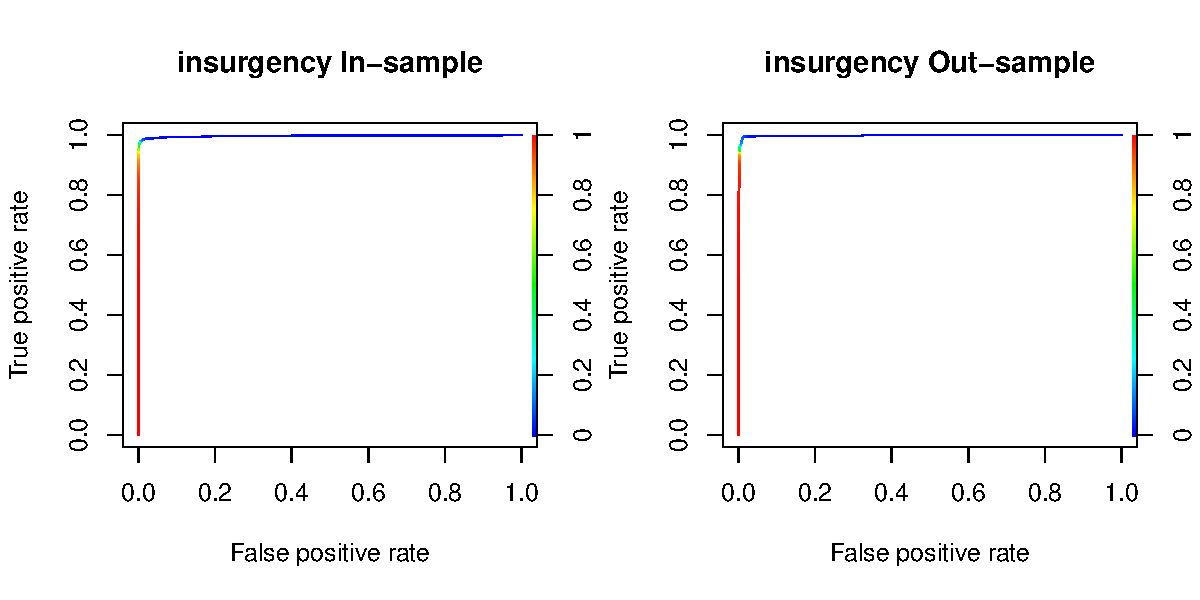
\includegraphics[width=\textwidth]{fig/roc_insurgency}
\end{figure}

\begin{figure}[H]
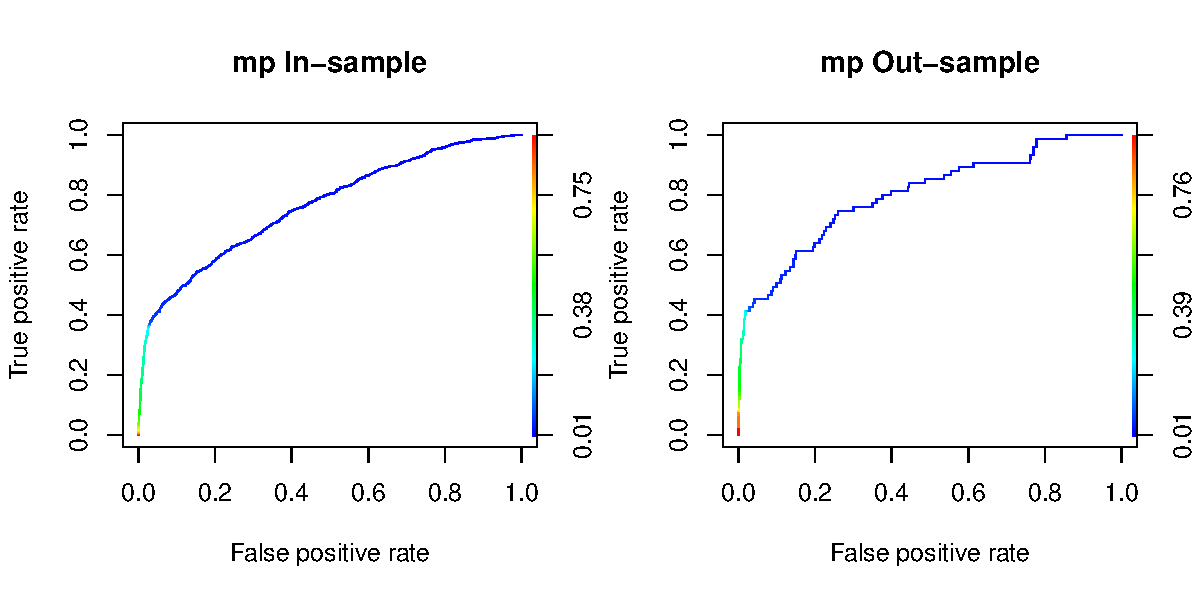
\includegraphics[width=\textwidth]{fig/roc_mp}
\end{figure}


\end{document}
